% Set a pdf version and a document type
\ifx\pdfminorversion\undefined\else\pdfminorversion=4\fi
\documentclass[aspectratio=169,t,table]{beamer}

% Import all necessary packages
% Use this file to import all packages which are needed for the lecture
\usepackage[english]{babel}
\usepackage[utf8]{inputenc}
\usepackage[sfdefault]{roboto}
\usepackage[T1]{fontenc}
\usepackage{amsmath,amssymb}
\usepackage{graphicx}
\usepackage{listings}
\usepackage[backend=biber,sorting=none,doi=true,style=ieee]{biblatex}
\usepackage{url}
\usepackage{hyperref}
\usepackage{fontawesome5}
\usepackage{graphicx}
\usepackage{booktabs}
\usepackage{calc}
\usepackage{ifthen}
\usepackage{tabularx}
\usepackage{longtable}
\usepackage{makecell}
\usepackage{multicol}
\usepackage{multirow}
\usepackage{hhline}
\usepackage{qrcode}
\usepackage{xcolor}
\usepackage{cleveref}
\usepackage{tikz}
\usepackage{tikz-cd}
\usepackage{pgfplots,pgfplotstable,pgf-pie}
\usepackage[linesnumbered]{algorithm2e}
\usepackage{array}
\usepackage{mathtools}
\usetikzlibrary{patterns}
\usetikzlibrary{arrows.meta}


% Set the theme (customized FAU beamer theme)
\usetheme[%
	image,%
	longtitle,%
	inst=tf%
]{fau}

% Set all important settings and define commands that are used in more than one lecture
% English version FAU Logo
\usepackage[english]{babel}
% German version FAU Logo
%\usepackage[ngerman]{babel}

\usepackage[utf8]{inputenc}
\usepackage[T1]{fontenc}
\usepackage{amsmath,amssymb}
\usepackage{graphicx}
\usepackage{listings}
\usepackage[backend=biber,sorting=none,doi=true,style=ieee]{biblatex}

% Options:
%  - inst:      Institute
%                 med:      MedFak FAU theme
%                 nat:      NatFak FAU theme
%                 phil:     PhilFak FAU theme
%                 rw:       RWFak FAU theme
%                 rw-jura:  RWFak FB Jura FAU theme
%                 rw-wiso:  RWFak FB WISO FAU theme
%                 tf:       TechFak FAU theme
%  - image:     Cover image on title page
%  - plain:     Plain title page
%  - longtitle: Title page layout for long title
\usetheme[%
	image,%
	longtitle,%
	inst=tf%
]{fau}

% Enable semi-transparent animation preview
\setbeamercovered{transparent}

% Enable frame numbering
%\setbeamertemplate{footline}[frame number]


\lstset{%
	language=Python,
	tabsize=2,
	basicstyle=\tt,
	keywordstyle=\color{blue},
	commentstyle=\color{green!50!black},
	stringstyle=\color{red},
	numbers=left,
	numbersep=0.5em,
	xleftmargin=1em,
	numberstyle=\tt
}

\defbibheading{bibliography}{}
\addbibresource{references.bib}

\date[SS2022]{Summer semester 2022}


\usepackage{url}
\usepackage{enumitem}
\setlist[itemize]{noitemsep, nolistsep}
\setlist[itemize]{label=\footnotesize\raisebox{.275ex}{$\bullet$}}
\usepackage{hyperref}
\usepackage{fontawesome5}
\usepackage{graphicx}
\usepackage{booktabs}
\usepackage{calc}
\usepackage{ifthen}

\usepackage{tabularx}
\usepackage{makecell}

\usepackage{xcolor}
\definecolor{airforceblue}{rgb}{0.36, 0.54, 0.66}
\definecolor{ForestGreen}{rgb}{0.34, 0.139, 0.34}

% English version
\institute[CS6]{Chair of Computer Science 6 (Data Management), Friedrich-Alexander University Erlangen-N\"urnberg}
% German version
% \institute[Lehrstuhl]{Lehrstuhl, Friedrich-Alexander-Universit\"at Erlangen-N\"urnberg}

\setbeamertemplate{section in toc}[sections numbered]

\setbeamertemplate{section page}{%
	\begingroup
	\begin{beamercolorbox}[sep=10pt,center,rounded=true,shadow=true]{section title}
		\usebeamerfont{section title}\thesection~\insertsection\par
	\end{beamercolorbox}
	\endgroup
}

\usepackage{tikz}
\usepackage{tikz-cd}
\usepackage{pgfplots,pgfplotstable,pgf-pie}

\newcommand{\tikzmark}[1]{\tikz[remember picture] \node[coordinate] (#1) {#1};}

\tikzset{
	every overlay node/.style={
			%draw=black,fill=white,rounded corners,
			anchor=north west, inner sep=0pt,
		},
}
% Usage:
% \tikzoverlay at (-1cm,-5cm) {content};
% or
% \tikzoverlay[text width=5cm] at (-1cm,-5cm) {content};
\def\tikzoverlay{%
	\tikz[remember picture, overlay]\node[every overlay node]
}%

\newcommand{\plots}{0.611201}
\newcommand{\plotm}{2.19882}

\newcommand{\MaxNumberX}{3}
\newcommand{\MaxNumberY}{5}

\pgfmathdeclarefunction{gauss}{2}{%
	\pgfmathparse{1/(#2*sqrt(2*pi))*exp(-((x-#1)^2)/(2*#2^2))}%
}

\tikzset{
	thick,
	>=latex,
	every edge/.style={draw=gray, thick, >=latex},
	vertex/.style = {
			circle,
			fill            = black,
			outer sep = 2pt,
			inner sep = 1pt,
		}
}
\usetikzlibrary{matrix,mindmap}
\usetikzlibrary{arrows,decorations.pathmorphing,backgrounds,fit,positioning,shapes.symbols,chains,intersections,snakes}
\tikzset{level 1/.append style={sibling angle=50,level distance = 165mm}}
\tikzset{level 2/.append style={sibling angle=20,level distance = 45mm}}
\tikzset{every node/.append style={scale=1}}
% read in data file
\pgfplotstableread{data/iris.dat}\iris
% get number of data points
\pgfplotstablegetrowsof{\iris}
\pgfmathsetmacro\NumRows{\pgfplotsretval-1}

\usepgfplotslibrary{groupplots}
\pgfplotsset{height=4cm,width=8cm,compat=1.14}

\tikzset{
	vertex/.style = {
			circle,
			fill            = black,
			outer sep = 2pt,
			inner sep = 1pt,
		}
}

\tikzset{
	mynode/.style={
			draw,
			thick,
			anchor=south west,
			minimum width=2cm,
			minimum height=1.3cm,
			align=center,
			inner sep=0.2cm,
			outer sep=0,
			rectangle split,
			rectangle split parts=2,
			rectangle split draw splits=false},
	reverseclip/.style={
			insert path={(current page.north east) --
					(current page.south east) --
					(current page.south west) --
					(current page.north west) --
					(current page.north east)}
		}
}

\tikzset{basic/.style={
			draw,
			rectangle split,
			rectangle split parts=2,
			rectangle split part fill={blue!20,white},
			minimum width=2.5cm,
			text width=2cm,
			align=left,
			font=\itshape
		},
	Diamond/.style={ diamond,
			draw,
			shape aspect=2,
			inner sep = 2pt,
			text centered,
			fill=blue!10!white,
			font=\itshape
		}}


\tikzset{level 1/.append style={sibling angle=50,level distance = 165mm}}
\tikzset{level 2/.append style={sibling angle=20,level distance = 45mm}}
\tikzset{every node/.append style={scale=1}}

\usetikzlibrary{arrows,decorations.pathmorphing,backgrounds,fit,positioning,shapes.symbols,chains,intersections,snakes,positioning,matrix,mindmap,shapes.multipart,shapes,calc,shapes.geometric}



% Title, author(s), and date
\title[KDDmUe~5.~OLAP]{5. Data Warehousing and Online Analytical Processing} %
\subtitle{Knowledge Discovery in Databases with Exercises}
\author[D.~Probst]{Dominik Probst, \texttt{dominik.probst@fau.de}}


% Metadata
\input{x-additional/vc.tex}
\hypersetup{
	pdftitle={KDDmUe - 5. Data Warehousing and Online Analytical Processing},
	pdfkeywords={
		KDD, 
		KDDmUe, 
		Knowledge Discovery in Databases, 
		Knowledge Discovery in Databases with Exercises, 
		FAU Erlangen-Nürnberg, 
		Data Science, 
		Machine Learning, 
		Data Mining, 
		Lecture, 
		Data Warehousing,
		OLAP,
		Data Cube,
		Star Schema,
		ETL,
		Extract, Transform, Load,
		OLAP Operations,
		Slice and Dice,
		Decision Support,
		Version \GITAbrHash
	},
	pdfsubject={Lecture on data warehousing and OLAP: covers data cube modeling, star schemas, ETL processes, and OLAP operations like slice and dice for decision support.},
	pdfcreator={Dominik Probst, CS6, FAU Erlangen-Nürnberg},
	pdflang={English}
}

% Define a custom column type
\newcolumntype{b}{>{\columncolor{faugray!62}}l}

% Start the document
\begin{document}

% Title
\maketitle

{ % Outline
	\setbeamertemplate{footline}{}
	\begin{frame}[noframenumbering]{Outline}
		\tableofcontents

	\end{frame}
}

% Body
\section{Data Warehouse: Basic Concepts}

\begin{frame}{What is a Data Warehouse?}
	William ``Bill'' H.  Inmon is commonly refered to as the ``father of the data warehouse''.
	\begin{block}{Data Warehouse\footnote{\fullcite{inmon2005}}}
		A data warehouse is a \textbf{subject-oriented}, \textbf{integrated}, \textbf{time-variant}, and \textbf{nonvolatile} collection of data in support of management's decision-making process.
	\end{block}

	\small
	\textbf{Other definitions exist:}
	\begin{itemize}
		\item ``A data warehouse is a system that extracts, cleans, conforms, and delivers source data into a dimensional data store and then supports and implements querying and analysis for the purpose of decision making.''\footnote{\fullcite{kimball2004}}
		\item A \textbf{\color{airforceblue}decision-support} database that is
		      \textbf{\color{airforceblue}maintained separately} from the organization's
		      operational database.
		\item Supports information processing by providing a solid platform of
		      \textbf{\color{airforceblue}consolidated, historical data} for analysis.
	\end{itemize}

	\textbf{\color{airforceblue}Data warehousing:} The process of constructing and using data warehouses.
\end{frame}

\begin{frame}{Data Warehouse -- Subject-oriented}
	\begin{itemize}
		\item \textbf{Organized around major subjects.} Such as customer, product,
		      sales.
		\item \textbf{Focusing on the modeling and analysis of data for
				      {\color{airforceblue}decision makers}.} Not on daily operations or
		      transaction processing.
		\item \textbf{Provide a simple and concise view around particular
			      subject issues.} By excluding data that are not useful in the
		      decision-support process.
	\end{itemize}
\end{frame}

\begin{frame}{Data Warehouse -- Integrated}
	\begin{itemize}
		\item \textbf{Constructed by {\color{airforceblue}integrating multiple heterogeneous data sources}.}
		      \begin{itemize}
			      \item Relational databases, flat files, online transaction records, \ldots
		      \end{itemize}
		\item \textbf{Data-cleaning and data-integration techniques are applied.}
		      \begin{itemize}
			      \item Ensure consistency in naming conventions, encoding structures, attribute measures, etc. among different data sources.
			      \item E.g., hotel price: currency, tax, breakfast covered, etc.
			      \item When data is moved to the warehouse, it is converted.
			      \item ETL -- Extraction, Transformation, Loading, see below.
		      \end{itemize}
	\end{itemize}
\end{frame}

\begin{frame}{Data Warehouse -- Time-Variant}
	\begin{itemize}
		\item \textbf{The {\color{airforceblue}time horizon} for a data warehouse is
				      {\color{airforceblue}significantly longer} than that of operational
			      systems.}
		      \begin{itemize}
			      \item Operational database: current-value data.
			      \item Data warehouse: provide information from a historical perspective, e.g. past $5-10$ years.
		      \end{itemize}
		\item \textbf{Every key structure in the data warehouse contains an
			      element of time, explicitly or implicitly.}
		\item The key of operational data may or may not contain a "time element."
	\end{itemize}
\end{frame}

\begin{frame}{Data Warehouse -- Nonvolatile}
	\begin{itemize}
		\item \textbf{A {\color{airforceblue}physically separate} store of data.}
		      \begin{itemize}
			      \item Transformed from the operational environment.
			      \item By {\color{airforceblue}copying}.
		      \end{itemize}
		\item \textbf{No operational update of data:}
		      \begin{itemize}
			      \item Hence, does not require transaction processing, \\
			            i.e. no logging, recovery, concurrency control, etc.
			      \item Requires only three operations:
			            \begin{enumerate}
				            \item Initial loading of data.
				            \item Refresh (update, often periodically, e.g. over night).
				            \item Access of data.
			            \end{enumerate}
		      \end{itemize}
	\end{itemize}
\end{frame}

\begin{frame}{Data Warehouse Usage}
	\textbf{Three kinds of data warehouse applications.}
	\begin{itemize}
		\item \textbf{\color{airforceblue}Information processing.}
		      \begin{itemize}
			      \item Supports querying, basic statistical analysis, and \\ reporting using crosstabs, tables, charts and graphs.
		      \end{itemize}
		\item \textbf{\color{airforceblue}Analytical processing.}
		      \begin{itemize}
			      \item Multidimensional analysis of data warehouse data.
			      \item Supports basic OLAP operations, slice-dice, drilling, pivoting.
		      \end{itemize}
		\item \textbf{\color{airforceblue}Data mining.}
		      \begin{itemize}
			      \item Knowledge discovery from hidden patterns.
			      \item Supports associations, constructing analytical models, performing classification and prediction, and presenting the mining results using visualization tools.
		      \end{itemize}
	\end{itemize}
\end{frame}


\begin{frame}{OLTP vs. OLAP}
	\begin{tabularx}{\textwidth}{|b|X|X|}
		\rowcolor{faugray!62}          & \textbf{OLTP}                                            & \textbf{OLAP}                                                      \\\hline
		\textbf{Users}                 & clerk, IT professional                                   & knowledge worker                                                   \\ \hline
		\textbf{Function}              & day-to-day operations                                    & decision support                                                   \\ \hline
		\textbf{DB Design}             & application-oriented                                     & decision support                                                   \\ \hline
		\textbf{Data}                  & current, up-to-date; detailed, flat relational; isolated & historical; summarized, multidimensional, integrated, consolidated \\ \hline
		\textbf{Usage}                 & repetitive                                               & ad-hoc                                                             \\ \hline
		\textbf{Access}                & read/write; index/hash on primary key                    & lots of scans                                                      \\ \hline
		\textbf{Unit of Work}          & short, simple transaction                                & complex query                                                      \\ \hline
		\textbf{$\#$-Records Accessed} & $~ 10$                                                   & $~ 10^6$                                                           \\ \hline
		\textbf{$\#$-Users}            & $~ 1000$                                                 & $~ 100$                                                            \\ \hline
		\textbf{DB Size}               & $~ 100$ MB to GB                                         & $~ 100$ GB to TB                                                   \\ \hline
		\textbf{Quantification}        & transaction throughput                                   & query throughput, response                                         \\ \hline
	\end{tabularx}
\end{frame}

\begin{frame}{Why a Separate Data Warehouse?}
	\textbf{High performance for both systems:}
	\begin{itemize}
		\item \textbf{\color{airforceblue}DBMS}: tuned for OLTP; Access methods,
		      indexing concurreny control, recovery.
		\item \textbf{\color{airforceblue}Warehouse}: tuned for OLAP; Complex OLAP
		      queries, multidimensional view, consolidation.
	\end{itemize}
	\textbf{Different functions and different data:}
	\begin{itemize}
		\item Missing data (DBMS):
		      \begin{itemize}
			      \item Decision support (DS) requires
			            \textbf{\color{airforceblue}historical data} which operational DBs do
			            not typically maintain.
		      \end{itemize}
		\item Data consolidation (warehouse):
		      \begin{itemize}
			      \item DS requires \textbf{\color{airforceblue}consolidation} (aggregation,
			            summarization) of data from heterogeneous sources.
		      \end{itemize}
		\item Data quality (warehouse):
		      \begin{itemize}
			      \item Different sources typically use inconsistent data representations,
			            codes and formats which have to be reconciled.
		      \end{itemize}
	\end{itemize}

	\textbf{Note: There are more and more systems which perform OLAP analysis
		directly on relational databases.}
\end{frame}

\begin{frame}{Three Data Warehouse Models}
	\begin{itemize}
		\item \textbf{\color{airforceblue}Enterprise warehouse:}
		      \begin{itemize}
			      \item Collects all of the information about subjects spanning the entire organization.
		      \end{itemize}
		\item \textbf{\color{airforceblue}Data mart:}
		      \begin{itemize}
			      \item A \textbf{\color{airforceblue}subset} of corporate-wide data that is of value to a \textbf{\color{airforceblue}specific group of users}.
			      \item Typically contains (highly) summarized data.
			      \item Independent vs. dependent (directly from warehouse) data mart.
		      \end{itemize}
		\item \textbf{\color{airforceblue}Virtual warehouse:}
		      \begin{itemize}
			      \item A set of \textbf{\color{airforceblue}views} over operational databases.
			      \item Only some of the possible summary views may be materialized.
		      \end{itemize}
	\end{itemize}
\end{frame}

\begin{frame}{Extraction, Transformation, and Loading (ETL)}
	\begin{itemize}
		\item \textbf{\color{airforceblue}Extraction:}
		      \begin{itemize}
			      \item Get data from multiple, heterogeneous, and external sources.
		      \end{itemize}
		\item \textbf{\color{airforceblue}Cleaning:}
		      \begin{itemize}
			      \item Detect errors in the data and rectify them if possible.
		      \end{itemize}
		\item \textbf{\color{airforceblue}Transformation:}
		      \begin{itemize}
			      \item Convert data from legacy or host format to warehouse format.
		      \end{itemize}
		\item \textbf{\color{airforceblue}Loading:}
		      \begin{itemize}
			      \item Sort, summarize, consolidate, compute views, check integrity, and build indexes and partitions.
		      \end{itemize}
		\item \textbf{\color{airforceblue}Refresh:}
		      \begin{itemize}
			      \item Propagate only the updates from the data sources to the warehouse.
		      \end{itemize}
	\end{itemize}
\end{frame}

\begin{frame}{Metadata\footnote{C.f. chapter 9 of \fullcite{kimball2004}} Repository}
	\begin{columns}
		\begin{column}{0.5\textwidth}
			Generally speaking:

			\begin{block}{Metadata}
				Data about data.
			\end{block}

			Three types: \textit{business}, \textit{process execution}, and
			\textit{technical} metadata.

			\vspace*{0.8em}
			\textbf{Business Metadata}
			\begin{itemize}
				\item Business terms and definitions.
				\item Logical data mapping.
				\item Data ownership.
				\item Charging policies.
			\end{itemize}
		\end{column}

		\begin{column}{0.5\textwidth}
			\textbf{Process Execution Metadata}
			\begin{itemize}
				\item Data acquisition schedule.
				\item Data-cleaning specifications.
				\item Aggregate specifications.
				\item Slowly changing dimensions policies.
				\item Duration of ETL, rows rejected and successfull.
			\end{itemize}
			\textbf{Technical Metadata}
			\begin{itemize}
				\item Table structures and table attributes.
				\item Derived data definitions.
				\item Results from data profiling.
				\item Data lineage.
			\end{itemize}

			\note{Data lineage = mapping of data and their tranformation process back
				to their originated source.}
		\end{column}
	\end{columns}
\end{frame}

% TODO: Insert (reference) architecture for data warehouse systems
% TODO: Insert requirements for data warehouse systems

\section{Data Warehouse Modeling: Data Cube and OLAP}

% TODO: Example ERM for sales

\begin{frame}{From Tables and Spreadsheets to Data Cubes}
	\begin{itemize}
		\item Data warehouse is based on a \textbf{\color{airforceblue}multidimensional data model} which views data in the form of a \textbf{data cube}.
		\item A {\color{faugray}\textbf{data cube}} allows data (example: sales) to be modeled and viewed in multiple dimensions.
		      \begin{itemize}
			      \item Defined by dimension and facts.
			      \item \textbf{Dimension tables:} such as: \texttt{item (item\_name, brand, type)},\\
			            or: \texttt{time (day, week, month, quarter, year)}.
			      \item \textbf{Fact table:} Contains \textbf{measures} (such as \texttt{dollars\_sold}) and references (\texttt{foreign keys}) to each of the related dimension tables.
		      \end{itemize}
		\item \textbf{$n$-dimensional base cube.}
		      \begin{itemize}
			      \item Called a base cuboid in data warehousing literature.
		      \end{itemize}
		\item \textbf{Top most $0$-dimensional cuboid.}
		      \begin{itemize}
			      \item Holds the highest-level of summarization.
			      \item Called the apex cuboid.
		      \end{itemize}
		\item \textbf{Lattice of cuboids.} (Forms a data cube)
	\end{itemize}
\end{frame}

\begin{frame}{Cube: A Lattice of Cuboids}
	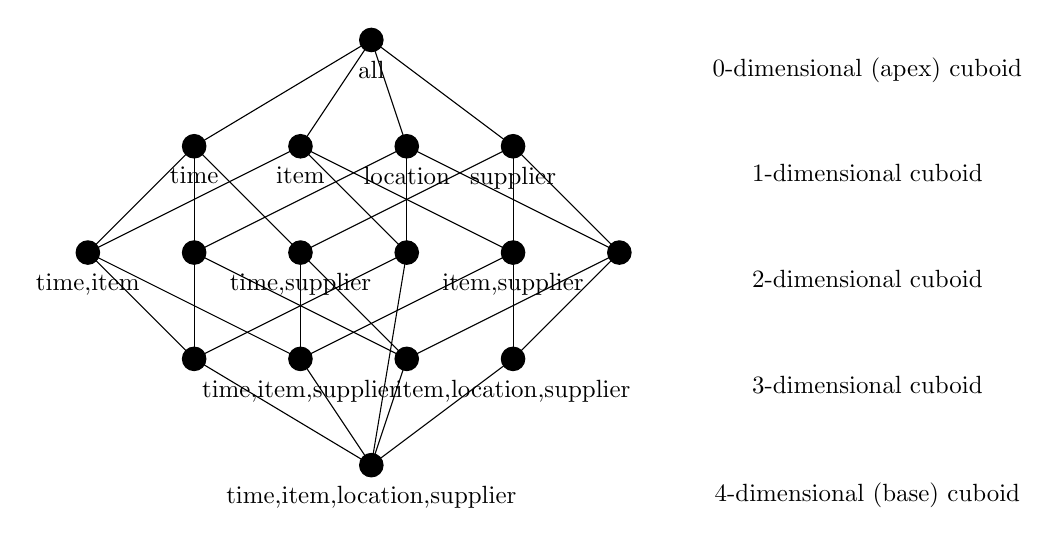
\begin{tikzpicture}[
			scale=0.9,
			every node/.style={transform shape},
		]
		\node[draw, circle, fill=black, label=below:{all}] at (2,6) {};
		\draw (2,6) -- (-0.5,4.5);
		\draw (2,6) -- (1,4.5);
		\draw (2,6) -- (2.5,4.5);
		\draw (2,6) -- (4,4.5);

		\node[draw, circle, fill=black, label=below:{time}] at (-0.5,4.5) {};
		\node[draw, circle, fill=black, label=below:{item}] at (1,4.5) {};
		\node[draw, circle, fill=black, label=below:{location}] at (2.5,4.5) {};
		\node[draw, circle, fill=black, label=below:{supplier}] at (4,4.5) {};

		\draw (-0.5,4.5) -- (-2,3);
		\draw (-0.5,4.5) -- (-0.5,3);
		\draw (-0.5,4.5) -- (1,3);
		\draw (1,4.5) -- (-2,3);
		\draw (1,4.5) -- (2.5,3);
		\draw (1,4.5) -- (4,3);
		\draw (2.5,4.5) -- (-0.5,3);
		\draw (2.5,4.5) -- (2.5,3);
		\draw (2.5,4.5) -- (5.5,3);
		\draw (4,4.5) -- (1,3);
		\draw (4,4.5) -- (4,3);
		\draw (4,4.5) -- (5.5,3);


		\node[draw, circle, fill=black, label=below:{time,item}] at (-2,3) {};
		\node[draw, circle, fill=black] at (-0.5,3) {};
		\node[draw, circle, fill=black, label=below:{time,supplier}] at (1,3) {};
		\node[draw, circle, fill=black] at (2.5,3) {};
		\node[draw, circle, fill=black, label=below:{item,supplier}] at (4,3) {};
		\node[draw, circle, fill=black] at (5.5,3) {};
		\draw (-2,3) -- (-0.5,1.5);
		\draw (-2,3) -- (1,1.5);
		\draw (-0.5,3) -- (-0.5,1.5);
		\draw (-0.5,3) -- (2.5,1.5);
		\draw (1,3) -- (1,1.5);
		\draw (1,3) -- (2.5,1.5);
		\draw (2.5,3) -- (-0.5,1.5);
		\draw (2.5,3) -- (2,0);
		\draw (4,3) -- (1,1.5);
		\draw (4,3) -- (4,1.5);
		\draw (5.5,3) -- (2.5,1.5);
		\draw (5.5,3) -- (4,1.5);

		\node[draw, circle, fill=black] at (-0.5,1.5) {};
		\node[draw, circle, fill=black, label=below:{time,item,supplier}] at (1,1.5) {};
		\node[draw, circle, fill=black] at (2.5,1.5) {};
		\node[draw, circle, fill=black, label=below:{item,location,supplier}] at (4,1.5) {};
		\draw (-0.5,1.5) -- (2,0);
		\draw (1,1.5) -- (2,0);
		\draw (2.5,1.5) -- (2,0);
		\draw (4,1.5) -- (2,0);

		\node[draw, circle, fill=black, label=below:{time,item,location,supplier}] at (2,0)  {};

		\node[label=below:{$0$-dimensional (apex) cuboid}] at (9,6)  {};
		\node[label=below:{$1$-dimensional cuboid}] at (9,4.5)  {};
		\node[label=below:{$2$-dimensional cuboid}] at (9,3)  {};
		\node[label=below:{$3$-dimensional cuboid}] at (9,1.5)  {};
		\node[label=below:{$4$-dimensional (base) cuboid}] at (9,0)  {};
	\end{tikzpicture}
\end{frame}

\begin{frame}{Conceptual Modeling of Data Warehouses}
	\begin{enumerate}
		\item \textbf{Star schema:}.
		      \begin{itemize}
			      \item A fact table in the middle connected to a set of dimension tables.
		      \end{itemize}
		\item \textbf{Snowflake schema:}.
		      \begin{itemize}
			      \item A refinement of the star schema where some dimensional hierarchies \\
			            are \textbf{normalized} into a set of smaller dimension tables,\\
			            forming a shape similar to a snowflake.
			      \item I. e. dimension tables of a star schema are split into multiple (dimension) tables\\ along their respective granularity level, but not split/normalized for every granularity.
		      \end{itemize}
		\item \textbf{Fact constellations:}.
		      \begin{itemize}
			      \item Multiple fact tables sharing dimension tables, \\
			            viewed as a collection of stars, therefore called \\
			            \textbf{galaxy schema} or fact constellation.
		      \end{itemize}
	\end{enumerate}
\end{frame}

\begin{frame}{Example of a Star Schema}
	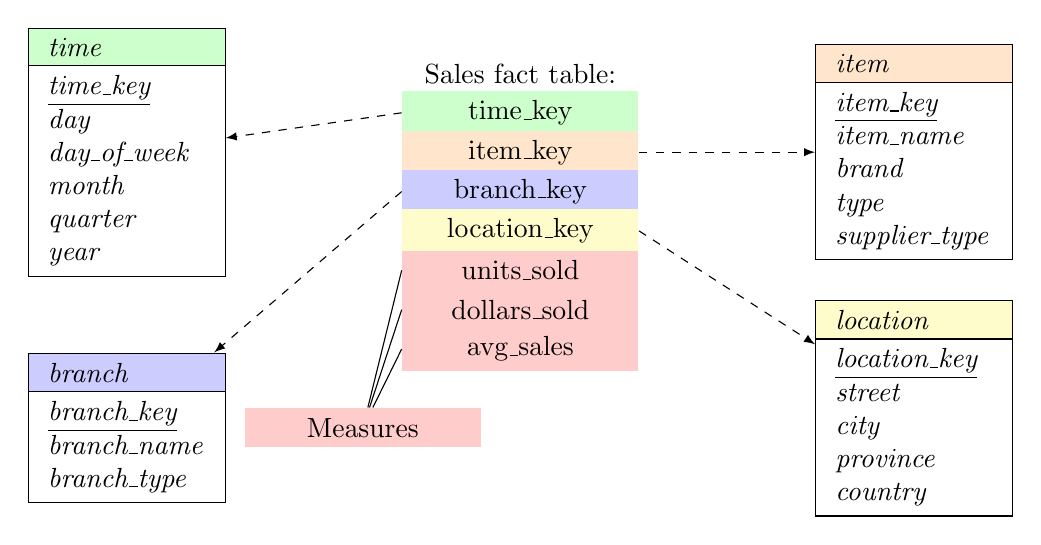
\begin{tikzpicture}
		\node[basic, rectangle split part fill={green!20,white}] at (2,2) (time) {time
			\nodepart{second}
			\underline{time\_key}\\
			day\\
			day\_of\_week\\
			month\\
			quarter\\
			year};

		\node[basic] at (2,-1.5) (branch) {branch
			\nodepart{second}
			\underline{branch\_key}\\
			branch\_name\\
			branch\_type};

		\node[basic, rectangle split part fill={orange!20,white}] at (12,2) (item) {item
			\nodepart{second}
			\underline{item\_key}\\
			item\_name\\
			brand\\
			type\\
			supplier\_type};

		\node[basic, rectangle split part fill={yellow!20,white}] at (12,-1.25) (location) {location
			\nodepart{second}
			\underline{location\_key}\\
			street\\
			city\\
			province\\
			country};

		\node[] at (7,3) {Sales fact table:};
		\node[fill=green!20, minimum width = 3cm, minimum height=0.5cm, align=right] at (7,2.5) (a) {time\_key};
		\node[fill=orange!20, minimum width = 3cm, minimum height=0.5cm, align=right] at (7,2) (b) {item\_key};
		\node[fill=blue!20, minimum width = 3cm, minimum height=0.5cm, align=right] at (7,1.5) (c) {branch\_key};
		\node[fill=yellow!20, minimum width = 3cm, minimum height=0.5cm, align=right] at (7,1) (d) {location\_key};
		\node[fill=red!20, minimum width = 3cm, minimum height=0.5cm, align=right] at (7,0.5) (units) {units\_sold};
		\node[fill=red!20, minimum width = 3cm, minimum height=0.5cm, align=right] at (7,0) (dollars) {dollars\_sold};
		\node[fill=red!20, minimum width = 3cm, minimum height=0.5cm, align=right] at (7,-0.5) (sales) {avg\_sales};
		\draw[->, dashed] (a.west) -- (time);
		\draw[->, dashed] (b) -- (item);
		\draw[->, dashed] (c.west) -- (branch);
		\draw[->, dashed] (d.east) -- (location);

		\node[fill=red!20, minimum width = 3cm, minimum height=0.5cm, align=right] at (5,-1.5) (e) {Measures};
		\draw[-] (e) -- (units.west);
		\draw[-] (e) -- (dollars.west);
		\draw[-] (e) -- (sales.west);
	\end{tikzpicture}
\end{frame}

\begin{frame}{Example of Snowflake Schema}
	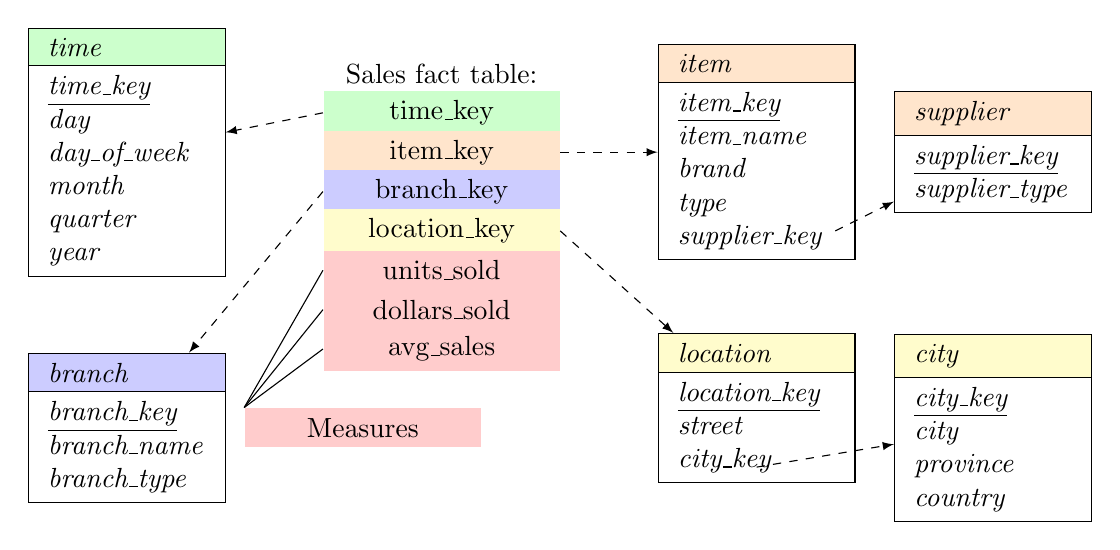
\begin{tikzpicture}
		\node[basic, rectangle split part fill={green!20,white}] at (2,2) (time) {time
			\nodepart{second}
			\underline{time\_key}\\
			day\\
			day\_of\_week\\
			month\\
			quarter\\
			year};

		\node[basic] at (2,-1.5) (branch) {branch
			\nodepart{second}
			\underline{branch\_key}\\
			branch\_name\\
			branch\_type};

		\node[basic, rectangle split part fill={orange!20,white}] at (10,2) (item) {item
			\nodepart{second}
			\underline{item\_key}\\
			item\_name\\
			brand\\
			type\\
			supplier\_key};

		\node[basic, rectangle split part fill={orange!20,white}] at (13,2) (supplier) {supplier
			\nodepart{second}
			\underline{supplier\_key}\\
			supplier\_type};

		\node[basic, rectangle split part fill={yellow!20,white}] at (10,-1.25) (location) {location
			\nodepart{second}
			\underline{location\_key}\\
			street\\
			city\_key};

		\node[basic, rectangle split part fill={yellow!20,white}] at (13,-1.5) (city) {city
			\nodepart{second}
			\underline{city\_key}\\
			city\\
			province\\
			country};

		\node[] at (6,3) {Sales fact table:};
		\node[fill=green!20, minimum width = 3cm, minimum height=0.5cm, align=right] at (6,2.5) (a) {time\_key};
		\node[fill=orange!20, minimum width = 3cm, minimum height=0.5cm, align=right] at (6,2) (b) {item\_key};
		\node[fill=blue!20, minimum width = 3cm, minimum height=0.5cm, align=right] at (6,1.5) (c) {branch\_key};
		\node[fill=yellow!20, minimum width = 3cm, minimum height=0.5cm, align=right] at (6,1) (d) {location\_key};
		\node[fill=red!20, minimum width = 3cm, minimum height=0.5cm, align=right] at (6,0.5) (units) {units\_sold};
		\node[fill=red!20, minimum width = 3cm, minimum height=0.5cm, align=right] at (6,0) (dollars) {dollars\_sold};
		\node[fill=red!20, minimum width = 3cm, minimum height=0.5cm, align=right] at (6,-0.5) (sales) {avg\_sales};
		\draw[->, dashed] (a.west) -- (time) ;
		\draw[->, dashed] (b) -- (item) ;
		\draw[->, dashed] (c.west) -- (branch) ;
		\draw[->, dashed] (d.east) -- (location) ;
		\draw[->, dashed] (10,-2) -- (city) ;
		\draw[->, dashed] (11,1) -- (supplier) ;

		\node[fill=red!20, minimum width = 3cm, minimum height=0.5cm, align=right] at (5,-1.5) (e) {Measures};
		\draw[-] (e.north west) -- (units.west);
		\draw[-] (e.north west) -- (dollars.west);
		\draw[-] (e.north west) -- (sales.west);
	\end{tikzpicture}
\end{frame}

\begin{frame}{Example of Fact Constellation}
	\vspace{-2.4em}
	\tikzset{basic/.style={
				draw,
				rectangle split,
				rectangle split parts=2,
				rectangle split part fill={blue!20,white},
				minimum width=2.5cm,
				text width=2cm,
				align=left,
				font=\itshape
			},
		Diamond/.style={ diamond,
				draw,
				shape aspect=2,
				inner sep = 2pt,
				text centered,
				fill=blue!10!white,
				font=\itshape
			}}
	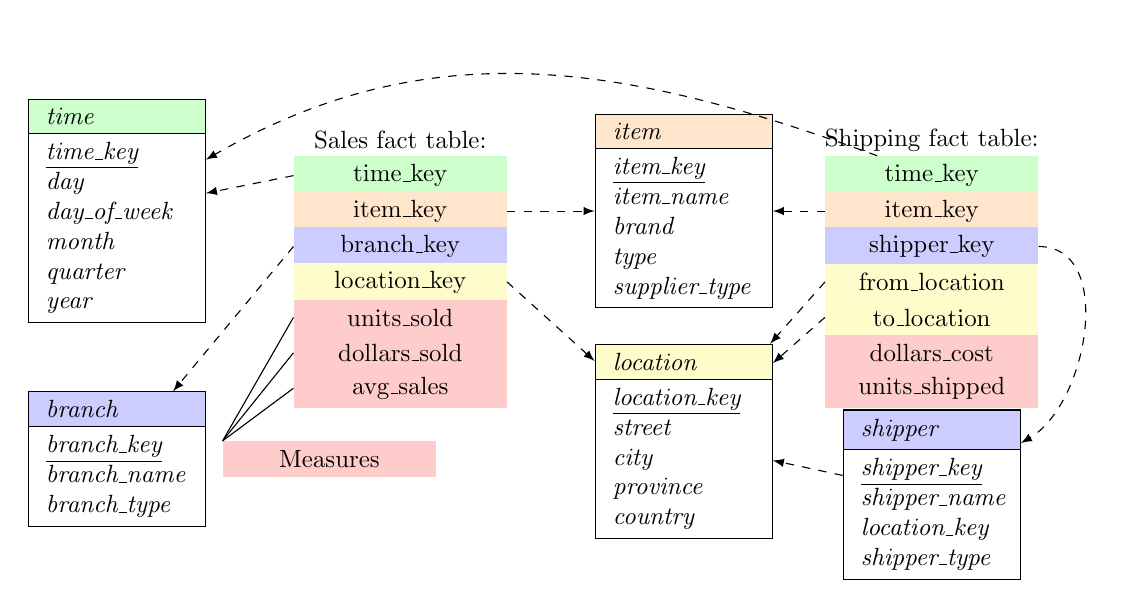
\begin{tikzpicture}[scale=0.9,every node/.style={transform shape}]
		\node[basic, rectangle split part fill={green!20,white}] at (2,2) (time) {time
			\nodepart{second}
			\underline{time\_key}\\
			day\\
			day\_of\_week\\
			month\\
			quarter\\
			year};

		\node[basic] at (2,-1.5) (branch) {branch
			\nodepart{second}
			\underline{branch\_key}\\
			branch\_name\\
			branch\_type};

		\node[basic, rectangle split part fill={orange!20,white}] at (10,2) (item) {item
			\nodepart{second}
			\underline{item\_key}\\
			item\_name\\
			brand\\
			type\\
			supplier\_type};

		\node[basic, rectangle split part fill={yellow!20,white}] at (10,-1.25) (location) {location
			\nodepart{second}
			\underline{location\_key}\\
			street\\
			city\\
			province\\
			country};

		\node[basic, rectangle split part fill={blue!20,white}] at (13.5,-2) (shipper) {shipper
			\nodepart{second}
			\underline{shipper\_key}\\
			shipper\_name\\
			location\_key\\
			shipper\_type};

		\node[] at (6,3) {Sales fact table:};
		\node[fill=green!20, minimum width = 3cm, minimum height=0.5cm, align=right] at (6,2.5) (a) {time\_key};
		\node[fill=orange!20, minimum width = 3cm, minimum height=0.5cm, align=right] at (6,2) (b) {item\_key};
		\node[fill=blue!20, minimum width = 3cm, minimum height=0.5cm, align=right] at (6,1.5) (c) {branch\_key};
		\node[fill=yellow!20, minimum width = 3cm, minimum height=0.5cm, align=right] at (6,1) (d) {location\_key};
		\node[fill=red!20, minimum width = 3cm, minimum height=0.5cm, align=right] at (6,0.5) (units) {units\_sold};
		\node[fill=red!20, minimum width = 3cm, minimum height=0.5cm, align=right] at (6,0) (dollars) {dollars\_sold};
		\node[fill=red!20, minimum width = 3cm, minimum height=0.5cm, align=right] at (6,-0.5) (sales) {avg\_sales};
		\draw[->, dashed] (a.west) -- (time) ;
		\draw[->, dashed] (b) -- (item) ;
		\draw[->, dashed] (c.west) -- (branch) ;
		\draw[->, dashed] (d.east) -- (location) ;


		\node[] at (13.5,3) {Shipping fact table:};
		\node[fill=green!20, minimum width = 3cm, minimum height=0.5cm, align=right] at (13.5,2.5) (q) {time\_key};
		\node[fill=orange!20, minimum width = 3cm, minimum height=0.5cm, align=right] at (13.5,2) (w) {item\_key};
		\node[fill=blue!20, minimum width = 3cm, minimum height=0.5cm, align=right] at (13.5,1.5) (e) {shipper\_key};
		\node[fill=yellow!20, minimum width = 3cm, minimum height=0.5cm, align=right] at (13.5,1) (r) {from\_location};
		\node[fill=yellow!20, minimum width = 3cm, minimum height=0.5cm, align=right] at (13.5,0.5) (t) {to\_location};
		\node[fill=red!20, minimum width = 3cm, minimum height=0.5cm, align=right] at (13.5,0) (z) {dollars\_cost};
		\node[fill=red!20, minimum width = 3cm, minimum height=0.5cm, align=right] at (13.5,-0.5) (u) {units\_shipped};
		\draw[->, dashed] (q) to [out=160,in=30] (time) ;
		\draw[->, dashed] (w) -- (item) ;
		\draw[->, dashed] (e.east) to [out=0,in=30] (shipper) ;
		\draw[->, dashed] (r.west) -- (location);
		\draw[->, dashed] (t.west) -- (location);
		\draw[->, dashed] (shipper) -- (location);

		\node[fill=red!20, minimum width = 3cm, minimum height=0.5cm, align=right] at (5,-1.5) (e) {Measures};
		\draw[-] (e.north west) -- (units.west);
		\draw[-] (e.north west) -- (dollars.west);
		\draw[-] (e.north west) -- (sales.west);
	\end{tikzpicture}
\end{frame}

\begin{frame}{A Concept Hierarchy: Dimension (Location)}
	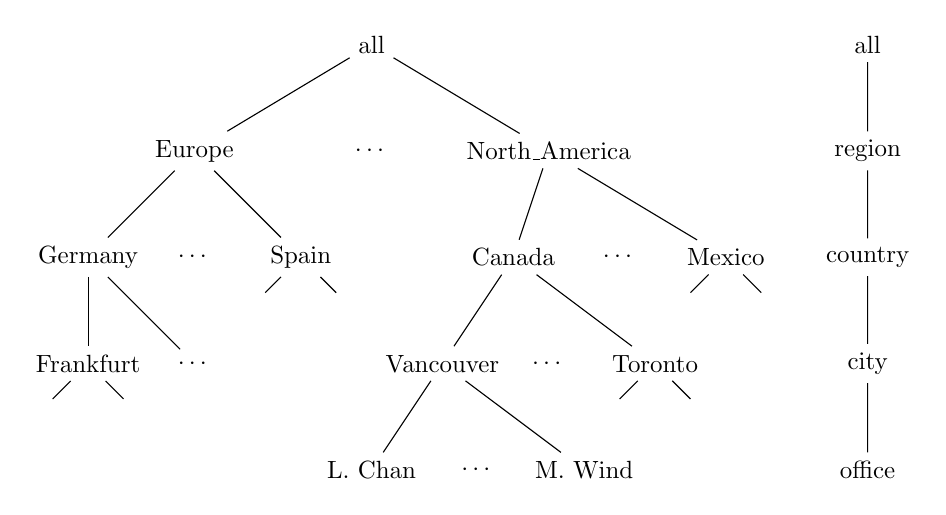
\begin{tikzpicture}[scale=0.9,every node/.style={transform shape}]
		\node at (2,6) (all) {all};

		\node at (-0.5,4.5) (europe) {Europe};
		\node at (2,4.5) (dot1) {$\cdots$};
		\node at (4.5,4.5) (america) {North\_America};

		\node at (-2,3) (germany) {Germany};
		\node at (-0.5,3) (dots2) {$\cdots$};
		\node at (1,3) (spain) {Spain};
		\node at (4,3) (canada) {Canada};
		\node at (5.5,3) (dots3) {$\cdots$};
		\node at (7,3) (mexico) {Mexico};

		\node at (-2,1.5) (frankfurt) {Frankfurt};
		\node at (-0.5,1.5) (dots4) {$\cdots$};
		\node at (3,1.5) (vancouver) {Vancouver};
		\node at (4.5,1.5) (dots5) {$\cdots$};
		\node at (6,1.5) (toronto) {Toronto};
		\node at (2,0) (lchan) {L. Chan};
		\node at (3.5,0) (dots6) {$\cdots$};
		\node at (5,0) (mwind) {M. Wind};

		\draw (all) -- (europe);
		\draw (all) -- (america);
		\draw (europe) -- (germany);
		\draw (europe) -- (spain);
		\draw (america) -- (canada);
		\draw (america) -- (mexico);
		\draw (germany) -- (frankfurt);
		\draw (germany) -- (dots4);
		\draw (spain) -- (0.5,2.5);
		\draw (spain) -- (1.5,2.5);
		\draw (mexico) -- (6.5,2.5);
		\draw (mexico) -- (7.5,2.5);
		\draw (frankfurt) -- (-2.5,1);
		\draw (frankfurt) -- (-1.5,1);
		\draw (toronto) -- (5.5,1);
		\draw (toronto) -- (6.5,1);
		\draw (canada) -- (vancouver);
		\draw (canada) -- (toronto);
		\draw (vancouver) -- (lchan);
		\draw (vancouver) -- (mwind);

		\node at (9,6) (all2) {all};
		\node at (9,4.5) (region2)  {region};
		\node at (9,3) (country2) {country};
		\node at (9,1.5) (city2) {city};
		\node at (9,0) (office2) {office};
		\draw (all2) -- (region2);
		\draw (region2) -- (country2);
		\draw (country2) -- (city2);
		\draw (city2) -- (office2);
	\end{tikzpicture}
\end{frame}

\begin{frame}{Data-Cube Measures}
	\begin{block}{Data-Cube Measure}
		A \textit{data-cube measure}, also called a \textit{fact}, is a numeric
		function that can be evaluated at each point in the data cube space.
	\end{block}

	\textbf{Three Categories:}
	\begin{enumerate}
		\item {\color{faugray}\textbf{Distributive:}}
		      \begin{itemize}
			      \item If the result derived by applying the function to the $n$ aggregate values obtained for $n$ partitions of the dataset is the same as that derived by applying the function on all the data without partitioning.\\
			            E.g. \texttt{COUNT, SUM, MIN, MAX}.
		      \end{itemize}
		\item {\color{faugray}\textbf{Algebraic:}}
		      \begin{itemize}
			      \item If it can be computed by an algebraic function with $M$ arguments, each of which is obtained by applying a distributive aggregate function.\\
			            E.g. \texttt{AVG, MIN$_N$, STD}.
		      \end{itemize}
		\item {\color{faugray}\textbf{Holistic:}}
		      \begin{itemize}
			      \item If there is no constant bound on the storage size needed to describe a subaggregate.\\
			            E.g. \texttt{MEDIAN, MODE, RANK}.
		      \end{itemize}
	\end{enumerate}
\end{frame}

\begin{frame}{Aggregation Type}
	\begin{itemize}
		\item \textbf{Non-trivial property.}
		      \begin{itemize}
			      \item Next to name and value range.
		      \end{itemize}
		\item \textbf{Defines the set of aggregation operations that can be executed on a measure (a fact).}
		\item \textbf{\color{airforceblue}FLOW:} Measure at a specific point in time.
		      \begin{itemize}
			      \item Aggregated as desired.
			      \item E.g. sales turnover, quantity of an item ordered per day.
		      \end{itemize}
		\item \textbf{\color{airforceblue}STOCK:} Measure over a period of time.
		      \begin{itemize}
			      \item Aggregated as desired, but temporal aggregation not permitted.
			      \item E.g. total stock and total inventory. Yet, summarization of article stock over multiple days makes no sense!
		      \end{itemize}
		\item \textbf{\color{airforceblue}VPU (Value per Unit):} Measures that cannot be summed.
		      \begin{itemize}
			      \item E.g. unit price, tax rates, exchange rates.
		      \end{itemize}
		\item \textbf{Always applicable: \texttt{MIN}, \texttt{MAX} and \texttt{AVG}.}
	\end{itemize}
\end{frame}

\begin{frame}{Aggregation Type}
	\textbf{Sales volume as a function of product, month, and region.}
	\begin{itemize}
		\item Dimensions: \texttt{Product, Location, Time.}
		\item Hierarchical summarization paths.
	\end{itemize}
	\vspace{0.5cm}
	\hspace{0.5cm}
	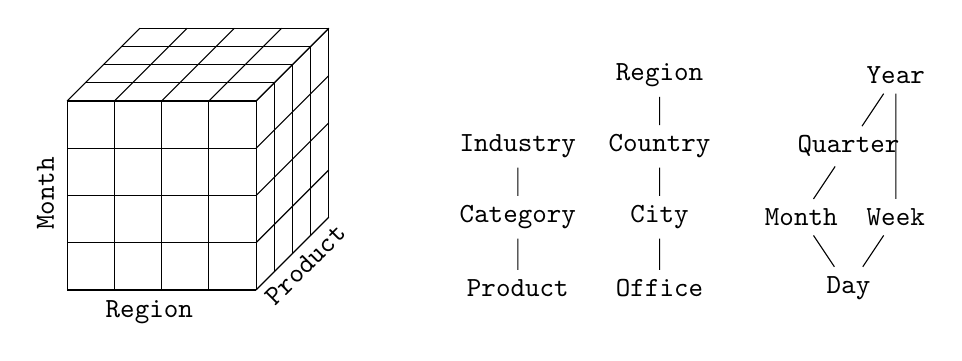
\begin{tikzpicture}[scale=0.6]
		\foreach \x in{0,...,4}
			{   \draw (0,\x ,4) -- (4,\x ,4);
				\draw (\x ,0,4) -- (\x ,4,4);
				\draw (4,\x ,4) -- (4,\x ,0);
				\draw (\x ,4,4) -- (\x ,4,0);
				\draw (4,0,\x ) -- (4,4,\x );
				\draw (0,4,\x ) -- (4,4,\x );
			}

		\node at (0.2,-2) {\texttt{Region}};
		\node[rotate=45] at (3.5,-1) {\texttt{Product}};
		\node[rotate=90] at (-2,0.5) {\texttt{Month}};

		\node at (8,1.5) (industry) {\texttt{Industry}};
		\node at (8,0) (category) {\texttt{Category}};
		\node at (8,-1.5) (product) {\texttt{Product}};
		\draw (industry) -- (category) -- (product);

		\node at (11,3) (region) {\texttt{Region}};
		\node at (11,1.5) (country) {\texttt{Country}};
		\node at (11,0) (city) {\texttt{City}};
		\node at (11,-1.5) (office) {\texttt{Office}};
		\draw (region) -- (country) -- (city) -- (office);

		\node at (16,3) (year) {\texttt{Year}};
		\node at (15,1.5) (quarter) {\texttt{Quarter}};
		\node at (14,0) (month) {\texttt{Month}};
		\node at (16,0) (week) {\texttt{Week}};
		\node at (15,-1.5) (day) {\texttt{Day}};
		\draw (year) -- (quarter) -- (month) -- (day) -- (week) -- (year);
	\end{tikzpicture}
\end{frame}

\begin{frame}{Data Cube Sample}
	\centering
	\includegraphics[width=10cm,height=6cm]{img/datacube.pdf}
\end{frame}

\begin{frame}{Cuboids Corresponding to the Cube}
	\centering
	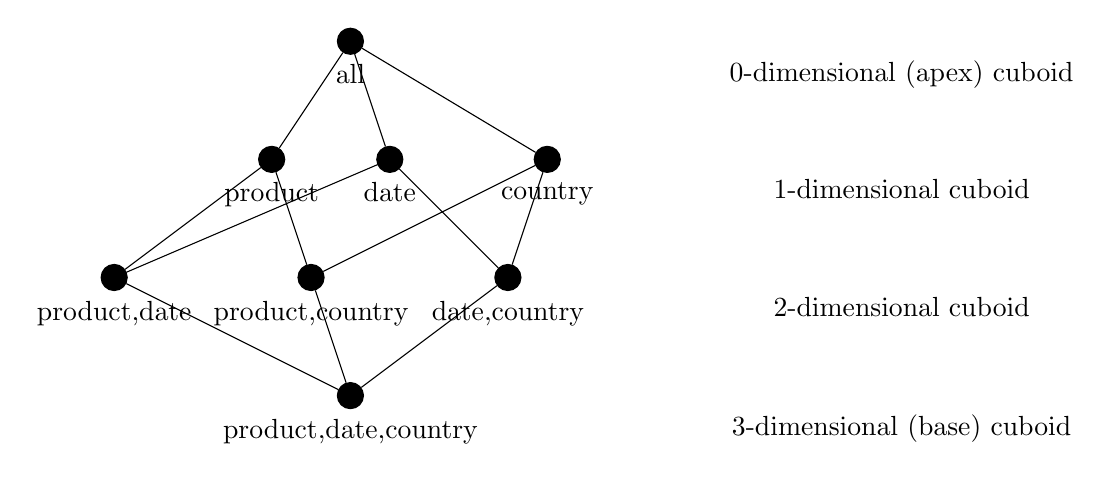
\begin{tikzpicture}
		\node[draw, circle, fill=black, label=below:{all}] at (2,6) (all) {};

		\node[draw, circle, fill=black, label=below:{product}] at (1,4.5) (product) {};
		\node[draw, circle, fill=black, label=below:{date}] at (2.5,4.5) (date) {};
		\node[draw, circle, fill=black, label=below:{country}] at (4.5,4.5) (country) {};

		\node[draw, circle, fill=black, label=below:{product,date}] at (-1,3) (productdate) {};
		\node[draw, circle, fill=black, label=below:{product,country}] at (1.5,3) (productcountry) {};
		\node[draw, circle, fill=black, label=below:{date,country}] at (4,3) (datecountry) {};

		\node[draw, circle, fill=black, label=below:{product,date,country}] at (2,1.5) (productdatecountry) {};

		\node[label=below:{$0$-dimensional (apex) cuboid}] at (9,6)  {};
		\node[label=below:{$1$-dimensional cuboid}] at (9,4.5)  {};
		\node[label=below:{$2$-dimensional cuboid}] at (9,3)  {};
		\node[label=below:{$3$-dimensional (base) cuboid}] at (9,1.5)  {};

		\draw (all) -- (product);
		\draw (all) -- (date);
		\draw (all) -- (country);
		\draw (product) -- (productdate);
		\draw (product) -- (productcountry);
		\draw (date) -- (productdate);
		\draw (date) -- (datecountry);
		\draw (country) -- (productcountry);
		\draw (country) -- (datecountry);
		\draw (productdate) -- (productdatecountry);
		\draw (productcountry) -- (productdatecountry);
		\draw (datecountry) -- (productdatecountry);
	\end{tikzpicture}
\end{frame}

\begin{frame}{Typical OLAP Operations}
	\begin{itemize}
		\item \textbf{{\color{airforceblue}Roll up} (drill up): summarize data.}
		      \begin{itemize}
			      \item By climbing up hierarchy or by dimension reduction.
		      \end{itemize}
		\item \textbf{{\color{airforceblue}Drill down} (roll down): reverse of roll up.}
		      \begin{itemize}
			      \item From higher-level summary to lower-level summary or detailed data, or introducing new dimensions.
		      \end{itemize}
		\item \textbf{{\color{airforceblue}Slice and dice}: project and select.}
		\item \textbf{{\color{airforceblue}Pivot} (rotate):}
		      \begin{itemize}
			      \item Reorient the cube, visualization, 3D to series of 2D planes.
		      \end{itemize}
		\item \textbf{Other operations:}
		      \begin{itemize}
			      \item \textbf{{\color{airforceblue}Drill across}:} involving (across) more than one fact table.
			      \item \textbf{{\color{airforceblue}Drill through}:} through the bottom level of the cube \\ to its back-end relational tables (using SQL).
		      \end{itemize}
	\end{itemize}
\end{frame}

\section{Data Warehouse Design and Usage}

\begin{frame}{Design of Data Warehouse: A Framework}
	\textbf{Four views regarding the design of a data warehouse:}
	\begin{itemize}
		\item \textbf{\color{airforceblue}Top-down view:}
		      \begin{itemize}
			      \item Allows selection of the relevant information necessary for the data warehouse.
		      \end{itemize}
		\item \textbf{\color{airforceblue}Data-source view:}
		      \begin{itemize}
			      \item Exposes the information being captured, stored, and managed by operational systems.
		      \end{itemize}
		\item \textbf{\color{airforceblue}Data warehouse view:}
		      \begin{itemize}
			      \item Consists of fact tables and dimension tables.
		      \end{itemize}
		\item \textbf{\color{airforceblue}Business-query view:}
		      \begin{itemize}
			      \item Sees the perspectives of data in the warehouse from the view of the end-user.
		      \end{itemize}
	\end{itemize}
\end{frame}

\begin{frame}{Data Warehouse Design Process}
	\vspace{-0.5em}
	\begin{itemize}
		\item \textbf{Top-down, bottom-up approaches or a combination of both:}
		      \begin{itemize}
			      \item \textbf{\color{airforceblue}Top-down:} starts with overall design and planning (mature).
			      \item \textbf{\color{airforceblue}Bottom-up:} starts with experiments and prototypes (rapid).
		      \end{itemize}
		\item \textbf{From software-engineering point of view:}
		      \begin{itemize}
			      \item \textbf{\color{airforceblue}Waterfall:} structured and systematic analysis at each step before proceeding to the next.
			      \item \textbf{\color{airforceblue}Spiral:} rapid generation of increasingly functional systems, short turn-around time.
		      \end{itemize}
		\item \textbf{Typical Data warehouse design process:}
		      \begin{enumerate}
			      \item Choose a \textbf{\color{airforceblue}business process} to model, e.g., orders, invoices, etc.
			      \item Choose a \textbf{\color{airforceblue}grain} (atomic level of data) of the business process.
			      \item Choose \textbf{\color{airforceblue}dimensions} that will apply to each fact-table record.
			      \item Choose a \textbf{\color{airforceblue}measure} that will populate each fact-table record.
		      \end{enumerate}
	\end{itemize}

	\begin{alertblock}{DWH Construction is No Easy Feat}
		Construction of a data warehouse is a difficult long-term task. It is absolutely necessary that its implementation scope is clearly defined at the beginning. Goals and tasks should be \textit{SMART} (specific, measurable, achievable, relevant, and time-related).
	\end{alertblock}
\end{frame}

\begin{frame}{Data Warehouse Development}
	\centering
	\begin{tikzpicture}[>=latex']
		\tikzset{block/.style= {draw, rectangle, align=center,minimum width=2cm,minimum height=1cm},
			rblock/.style={draw, shape=rectangle,rounded corners=1.5em,align=center,minimum width=2cm,minimum height=1cm},
			input/.style={ % requires library shapes.geometric
					draw,
					trapezium,
					trapezium left angle=60,
					trapezium right angle=120,
					minimum width=2cm,
					align=center,
					minimum height=1cm
				},
		}
		\node[block] at (2,2) (ddm) {Distributed data marts};
		\node[block] at (8,3) (mtier) {Multi-tier data warehouse};

		\node[block] at (0.5,0) (datamart1) {Data mart};
		\node[block] at (3.5,0) (datamart2) {Data mart};
		\node[block] at (8,0) (edw) {Enterprise data warehouse};
		\node[block] at (5,-2) (hlw) {Define a high-level corporate data model};

		\path[draw,->] (hlw) edge (datamart1);
		\path[draw,->] (hlw) edge (datamart2);
		\path[draw,->,dashed] (datamart1) edge [bend right=30,faugraydark] (hlw);
		\path[draw,->,dashed] ($(datamart2.south)+(0.2,0)$) edge [faugraydark] ($(hlw.north)+(-0.55,0)$);
		\path[draw,->,dashed] (ddm) edge [bend left = 50,faugraydark] (hlw);
		\path[draw,->,dashed] (edw) edge [bend left = 40,faugraydark] (hlw);
		\path[draw,->] (datamart1) edge (ddm);
		\path[draw,->] (datamart2) edge (ddm);
		\path[draw,->] (ddm) edge (mtier);
		\path[draw,->] (edw) edge (mtier);
		\path[draw,->] (hlw) edge (edw);

		\path[draw,->,dashed,faugraydark] (0,3.5) -- node[below] {Model Refinement} (2,3.5);
	\end{tikzpicture}
\end{frame}

\section{Data Warehouse and Data Mining}


\begin{frame}{From Online Analytical Processing (OLAP) To Online Analytical Mining (OLAM)}
	\textbf{Why online analytical mining?}
	\begin{itemize}
		\item DW contains integrated, consistent, cleaned data.
		\item Available information-processing structure surrounding data warehouses.
		      \begin{itemize}
			      \item ODBC, OLEDB, Web access, service facilities, reporting, and OLAP tools.
		      \end{itemize}
		\item OLAP-based exploratory data analysis.
		      \begin{itemize}
			      \item Mining with drilling, dicing, pivoting, etc.
		      \end{itemize}
		\item Online selection of data-mining functions.
		      \begin{itemize}
			      \item Integration and swapping of multiple mining functions, algorithms, and tasks.
		      \end{itemize}
	\end{itemize}
\end{frame}


\begin{frame}{Data Warehouse and Data Mining}
	\vspace*{-1em}
	\begin{tikzpicture}[
		scale=0.8,
		every node/.style={transform shape},
		>=latex,
		thick,
		node distance=2em,
		database/.style={
				cylinder,
				cylinder uses custom fill,
				shape border rotate=90,
				aspect=0.25,
				draw,
				align=center
			}
	]
	\node[database,text width=4em] (source1) at (0,0) {ERP};
	\node[database,below=1em of source1,text width=4em] (source2) {CRM};
	\node[database,below=1em of source2,text width=4em] (source3) {MES};
	\node[database,below=1em of source3,text width=4em] (source4) {\dots};

	\node[signal,minimum width=4em,minimum height=1cm,draw=black,below right=-0.5em and 16em of source2,fill=faured!75] (load) {\hspace*{1.5em}Load};
	\node[signal,minimum width=4em,minimum height=1cm,draw=black,left=-1.6em of load,fill=fauorange] (transform) {\hspace*{1.5em}Transform};
	\node[signal,minimum width=4em,minimum height=1cm,draw=black,left=-1.6em of transform,fill=fauyellow] (extract) {Extract};

	\node[database,right=3em of load,text width=10em,fill=faucyan!75] (dwh) {\huge Data\\\smallskip\huge Warehouse};

	\node[database,right=5em of dwh,text width=4em,fill=faucyan!12] (dm2) {Data Mart 2};
	\node[database,above=2em of dm2,text width=4em,fill=faucyan!12] (dm1) {Data Mart 1};
	\node[database,below=2em of dm2,text width=4em,fill=faucyan!12] (dm3) {Data Mart $n$};

	\draw[->] ([yshift=1mm]source1.east) to[out=0,in=180] (extract.west);
	\draw[->] ([yshift=1mm]source2.east) to[out=0,in=180] (extract.west);
	\draw[->] ([yshift=1mm]source3.east) to[out=0,in=180] (extract.west);
	\draw[->] ([yshift=1mm]source4.east) to[out=0,in=180] (extract.west);

	\draw[->] (load) to (dwh);

	\draw[->] (dwh.east) to[out=0,in=180] (dm1.west);
	\draw[->] (dwh.east) to[out=0,in=180] (dm2.west);
	\draw[->] (dwh.east) to[out=0,in=180] (dm3.west);

	\node[above right=-2.8em and 6em of dm1] (analytics1) {\huge\faChartPie};
	\node[below=2em of analytics1] (analytics2) {\huge\faChartLine};
	\node[below=2em of analytics2] (analytics3) {\huge\faChartBar};
	\node[below=2em of analytics3] (analytics4) {\huge\faChartArea};

	\foreach \i in {1,...,4}
		{
			\foreach \j in {2,...,3}
				{
					\draw[gray,->] (dm\j) to[out=0,in=180] (analytics\i);
				}
		}

	\foreach \i in {1,...,4}
		{
			\draw[->] (dm1) to[out=0,in=180] (analytics\i);
		}
\end{tikzpicture}


	\begin{itemize}
		\item Data mining algorithms in transformation step: E.g. integrate articles from two systems that have different article group hierarchy. Goal: Map one article group hierarchy to the existing article group hierarchy.
		\item Frequent pattern mining and clustering in reporting: E.g. affinity
		      analysis, revenue prediction, cluster customers and use this insight for a
		      new marketing campaign.
	\end{itemize}
\end{frame}

\section{Summary}


\begin{frame}{Summary}
	\begin{itemize}
		\item \textbf{Data warehousing: multi-dimensional model of data.}
		      \begin{itemize}
			      \item A data cube consists of dimensions and measures.
			      \item Star schema, snowflake schema, fact constellations.
			      \item OLAP operations: drilling, rolling, slicing, dicing and pivoting.
		      \end{itemize}
		\item \textbf{Data warehouse architecture, design, and usage.}
		      \begin{itemize}
			      \item Multi-tiered architecture.
			      \item Business-analysis design framework.
			      \item Information processing, analytical processing, data mining, OLAM (Online Analytical Mining).
		      \end{itemize}
	\end{itemize}
\end{frame}


\begin{frame}{Interested in More Information?}
	Our appendix in this document covers:
	\begin{itemize}
		\item \textbf{Implementation: efficient computation of data cubes.}
		      \begin{itemize}
			      \item Partial vs. full vs. no materialization.
			      \item Indexing OLAP data: Bitmap index and join index.
			      \item OLAP query processing.
			      \item OLAP servers: ROLAP, MOLAP, HOLAP.
		      \end{itemize}
		\item \textbf{Data generalization: attribute-oriented induction.}
	\end{itemize}

	Additionally, check out these books:
	\begin{itemize}
		\item \fullcite{kimball2004}
		\item \fullcite{inmon2005}
		\item In German: \fullcite{bauer2013}
	\end{itemize}
\end{frame}

\begin{frame}[c]
	\begin{center}
		{\bf Any questions about this chapter?}\\[0.5cm]
		Ask them now or ask them later in our forum: \\\bigskip
		\qrcode{https://www.studon.fau.de/studon/goto.php?target=lcode_OLYeD79h} \\
		\vspace*{0.5cm}
		\faLink\ \url{https://www.studon.fau.de/studon/goto.php?target=lcode_OLYeD79h} \smallskip

	\end{center}
\end{frame}

\section{Appendix}
\appendix
\section{Data Warehouse Implementation}

\begin{frame}{Efficient Data-Cube Computation}
	\begin{itemize}
		\item \textbf{Data cube can be viewed as a lattice of cuboids.}
		\item The bottom-most cuboid is the base cuboid.
		\item The top-most cuboid (apex) contains only one cell.
		\item How many cuboids in an $n$-dimensional cube with $L_i$ levels associated with dimension $i$?
		      \begin{align}
			      T = \prod_{i=1}^{n} (L_i +1).
		      \end{align}
		\item \textbf{{\color{airforceblue}Materialization} of data cube.}
		      \begin{itemize}
			      \item Materialize each (cuboid) (full materialization), \\
			            none (no materialization), or some (partial materialization).
			      \item Selection of cuboids to materialize based on size, sharing, access frequency, etc.
		      \end{itemize}
	\end{itemize}
\end{frame}

\begin{frame}{The "Compute Cube" Operator}
	\begin{columns}
		\begin{column}{0.6\textwidth}
			\vspace{-4.8cm}
			\begin{itemize}
				\item \textbf{Cube definition and computation in DMQL:} \\
				      \texttt{DEFINE CUBE sales [item, city, year]:}\\
				      \texttt{SUM (sales$\_$in$\_$dollars);}\\
				      \texttt{COMPUTE CUBE sales;}
				\item \textbf{Transform it into an SQL-like language:}\\
				      with a new operator \texttt{CUBE BY} (Gray et al. 96).\\
				      \texttt{SELECT item, city, year, SUM (amount)}\\
				      \texttt{FROM sales}\\
				      \texttt{CUBE BY item, city, year;}
				\item \textbf{Need to compute the following} \texttt{GROUP BY}\textbf{s:}\\
				      \texttt{(city, item, year),}\\
				      \texttt{(city, item), (city, year),}\\
				      \texttt{(item, year),}\\
				      \texttt{(city), (item), (year)}\\
				      \texttt{()}
			\end{itemize}
		\end{column}
		\begin{column}{0.3\textwidth}  %%<--- here
			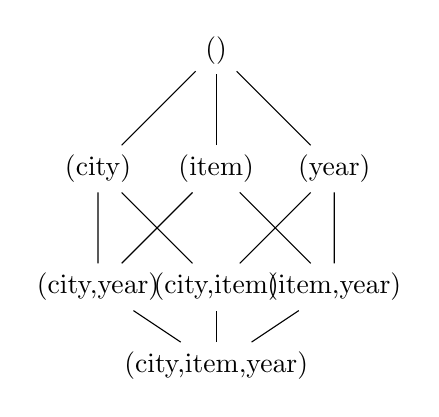
\begin{tikzpicture}
				\node at (0,0) (a) {()};
				\node at (0,-1.5) (b) {(item)};
				\node at (-1.5,-1.5) (c) {(city)};
				\node at (1.5,-1.5) (d) {(year)};
				\node at (0,-3) (e) {(city,item)};
				\node at (-1.5,-3) (f) {(city,year)};
				\node at (1.5,-3) (g) {(item,year)};
				\node at (0,-4) (h) {(city,item,year)};
				\draw (a) -- (c) -- (f) -- (h);
				\draw (h) -- (g) -- (d) -- (a);
				\draw (h) -- (e);
				\draw (e) -- (c);
				\draw (e) -- (d);
				\draw (f) -- (b);
				\draw (g) -- (b);
				\draw (b) -- (a);
			\end{tikzpicture}
		\end{column}
	\end{columns}
\end{frame}

\begin{frame}{Indexing OLAP Data: Bitmap Index}
	\begin{itemize}
		\item \textbf{Index on a particular column.}
		\item \textbf{Each value in the column has a bit vector: bit-op is fast.}
		\item \textbf{Length of bit vector: $\#$ of records in base table.}
		\item \textbf{$i$-th bit set, if $i$-th row of base table has value of bit vector.}
		\item \textbf{Not suitable for high-cardinality domains:}
		      \begin{itemize}
			      \item A bit compression technique called Word-Aligned Hybrid (WAH) makes it work for high-cardinality domain as well [Wu et al., TODS'06].
		      \end{itemize}
	\end{itemize}
	\centering
	\textbf{Base table} \hspace{2.5cm} \textbf{Index on region} \hspace{2.5cm} \textbf{Index on type}\\
	\begin{tabular}{| c | c | c |}
		\hline
		\textbf{Cust} & \textbf{Region} & \textbf{Type} \\\hline
		$C1$          & Asia            & Retail        \\\hline
		$C2$          & Europe          & Dealer        \\\hline
		$C3$          & Asia            & Dealer        \\\hline
		$C4$          & America         & Retail        \\\hline
		$C5$          & Europe          & Dealer        \\\hline
	\end{tabular}\hspace{0.1cm}
	\begin{tabular}{| c | c | c | c |}
		\hline
		\textbf{RecID} & \textbf{Asia} & \textbf{Europe} & \textbf{America} \\\hline
		1              & 1             & 0               & 0                \\\hline
		2              & 0             & 1               & 0                \\\hline
		3              & 1             & 0               & 0                \\\hline
		4              & 0             & 0               & 1                \\\hline
		5              & 0             & 1               & 0                \\\hline
	\end{tabular}\hspace{0.1cm}
	\begin{tabular}{| c | c | c |}
		\hline
		\textbf{RecID} & \textbf{Retail} & \textbf{Dealer} \\\hline
		$1$            & 1               & 0               \\\hline
		$2$            & 0               & 1               \\\hline
		$3$            & 0               & 1               \\\hline
		$4$            & 1               & 0               \\\hline
		$5$            & 0               & 1               \\\hline
	\end{tabular}
\end{frame}

\begin{frame}{Indexing OLAP Data: Join Indices}
	\begin{itemize}
		\item \textbf{Join index:}
		      \begin{align}
			      \text{JI}(\texttt{R-id}, \texttt{S-id}) \quad \text{where} \quad \text{R}(\texttt{R-id}, \ldots) \bowtie  \text{S}(\texttt{S-id}, \ldots).
		      \end{align}
		\item \textbf{Traditional indices map the values to a list of record ids.}
		      \begin{itemize}
			      \item Materializes relational join in JI-file and speeds it up.
		      \end{itemize}
		\item \textbf{In data warehouses, join index relates the values of the dimensions \\ of a star schema to rows in the fact table.}
		      \begin{itemize}
			      \item E.g. fact table: Sales and two dimensions location and item.
			            \begin{itemize}
				            \item A join index on location maintains for each distinct location a list of \texttt{R-ids} of the tuples recording the sales in that location.
			            \end{itemize}
			      \item Join indices can span multiple dimensions.
		      \end{itemize}
	\end{itemize}
\end{frame}

\begin{frame}{Indexing OLAP data: Join Indices (Example)}
	\centering
	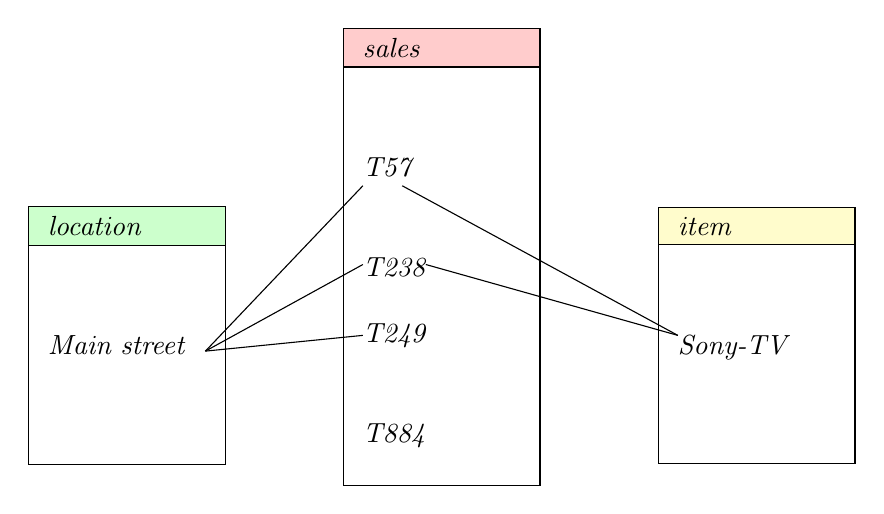
\begin{tikzpicture}
		\node[basic, rectangle split part fill={red!20,white}] at (2,2) (sales) {sales
			\nodepart{second}
			~\\
			~\\
			~\\
			T57\\
			~\\
			~\\
			T238
			~\\
			~\\
			T249
			~\\
			~\\
			~\\
			T884\\
			~};

		\node[basic, rectangle split part fill={green!20,white}] at (-2,1) (location) {location
			\nodepart{second}
			~\\
			~\\
			~\\
			Main street\\
			~\\
			~\\
			~};

		\node[basic, rectangle split part fill={yellow!20,white}] at (6,1) (item) {item
			\nodepart{second}
			~\\
			~\\
			~\\
			Sony-TV\\
			~\\
			~\\
			~};

		\draw (-1,0.8) -- (1,1);
		\draw (-1,0.8) -- (1,1.9);
		\draw (-1,0.8) -- (1,2.9);

		\draw (5,1) -- (1.5,2.9);
		\draw (5,1) -- (1.8,1.9);
	\end{tikzpicture}
\end{frame}

\begin{frame}{Efficient Processing of OLAP Queries}
	\begin{itemize}
		\item \textbf{Determine which operations should be performed on the available cuboids.}
		      \begin{itemize}
			      \item Transform drill, roll, etc. into corresponding SQL and/or OLAP operations.\\
			            E.g. \texttt{dice} $=$ \texttt{selection} $+$ \texttt{projection}.
		      \end{itemize}
		\item \textbf{Determine which materialized cuboid(s) should be selected for OLAP operation.}
		      \begin{itemize}
			      \item Let the query to be processed be on \texttt{\{brand, province\_or\_state\}} with the condition \texttt{"year = 2004"}, and there are $4$ materialized cuboids available:
			            \begin{itemize}
				            \item[1)] \texttt{{year, item\_name, city}}.
				            \item[2)] \texttt{{year, brand, country}}.
				            \item[3)] \texttt{{year, brand, province\_or\_state}}.
				            \item[4)] \texttt{{item\_name, province\_or\_state} where year $=$ 2004}.
			            \end{itemize}
			      \item Which should be selected to process the query?
		      \end{itemize}
		\item \textbf{Explore indexing structures and compressed vs. dense-array structures in MOLAP.}
	\end{itemize}
\end{frame}

\begin{frame}{OLAP Server Architectures}
	\begin{itemize}
		\item \textbf{Relational OLAP (ROLAP).}
		      \begin{itemize}
			      \item Use relational or extended-relational DBMS to store \\
			            and manage warehouse data and OLAP middleware.
			      \item Include optimization of DBMS backend, implementation of aggregation navigation logic, and additional tools and services.
			      \item Greater scalability.
		      \end{itemize}
		\item \textbf{Multidimensional OLAP (MOLAP).}
		      \begin{itemize}
			      \item Sparse array-based multidimensional storage engine.
			      \item Fast indexing to pre-computed summarized data.
		      \end{itemize}
		\item \textbf{Hybrid OLAP (HOLAP) (e.g., Microsoft SQL-Server).}
		      \begin{itemize}
			      \item Flexibility, e.g., low level: relational, high-level: array.
		      \end{itemize}
		\item \textbf{Specialized SQL servers (e.g., Redbricks).}
		      \begin{itemize}
			      \item Specialized support for SQL queries over star/snowflake schemas.
		      \end{itemize}
	\end{itemize}
\end{frame}

\section{Data Generalization by Attribute-Oriented Induction}

\begin{frame}{Data Generalization}
	\begin{itemize}
		\item \textbf{Summarize data:}
		      \begin{itemize}
			      \item \textbf{By replacing relatively low-level values} \\
			            e.g. numerical values for the attribute \texttt{age} \\
			            \textbf{with higher-level concepts}\\
			            e.g. \texttt{young}, \texttt{middle-aged} and \texttt{senior}.
			      \item \textbf{By reducing the number of dimensions}\\
			            e.g. removing \texttt{birth\_date} and \texttt{telephone\_number} \\ when summarizing the behavior of a group of students.
			      \item Describe concepts in concise and succinct terms at generalized (rather than low) levels of abstractions:
			            \begin{itemize}
				            \item Facilitates users in examining the general behavior of the data.
				            \item Makes dimensions of a data cube easier to grasp.
			            \end{itemize}
		      \end{itemize}
	\end{itemize}
\end{frame}

\begin{frame}{Attribute-Oriented Induction}
	\begin{itemize}
		\item \textbf{Proposed in 1989} (KDD'89 workshop).
		\item \textbf{Not confined to categorical data nor to particular measures.}
		\item \textbf{How is it done?}
		      \begin{itemize}
			      \item Collect the \textbf{\color{airforceblue}task-relevant data} (initial relation) using a relational database query.
			      \item Perform \textbf{\color{airforceblue}generalization} by attribute removal or attribute generalization.
			      \item Apply \textbf{\color{airforceblue}aggregation} by merging identical, generalized tuples and \\ accumulating their respective counts.
			      \item Interaction with users for knowledge presentation.
		      \end{itemize}
	\end{itemize}
\end{frame}

\begin{frame}{Attribute-Oriented Induction: An Example}
	\begin{itemize}
		\item \textbf{Example:} Describe general characteristics of graduate students in a university database.
		\item \textbf{Step 1:} Fetch relevant set of data using an SQL statement, e.g.\\[0.1cm]
		      \texttt{SELECT name, gender, major, birth\_place, birth\_date, residence, phone\#, gpa}\\
		      \texttt{FROM student}\\
		      \texttt{WHERE student\_status IN {"Msc", "MBA", "PhD"};}\\[0.1cm]
		\item \textbf{Step 2:} Perform attribute-oriented induction.
		\item \textbf{Step 3:} Present results in generalized-relation, cross-tab, or rule forms.
	\end{itemize}
\end{frame}

\begin{frame}{Class Characterization (I)}
	\begin{table}
		\small
		\begin{tabularx}{\textwidth}{|X|X|X|X|X|X|X|X|}
			\hline
			\textbf{Name}        & \textbf{Gender}       & \textbf{Major}             & \textbf{Birth place}         & \textbf{Birth date}    & \textbf{Residence}       & \textbf{Phone number} & \textbf{GPA}                 \\\hline
			Jim                  & M                     & CS                         & Vancouver, BC, Canada        & 08-21-76               & 3511 Main St., Richmond  & 687-4598              & 3.67                         \\\hline
			Scott Lachance       & M                     & CS                         & Montreal, Que, Canada        & 28-07-75               & 345 1st Ave., Richmond   & 253-9106              & 3.70                         \\\hline
			Laura Lee            & F                     & Physics                    & Seattle, WA, USA             & 25-08-70               & 125 Austin Ave., Burnaby & 420-5232              & 3.83                         \\\hline
			{\color{red}Removed} & {\color{red}Retained} & {\color{red}Sci, Eng, Bus} & {\color{red}Canada, Foreign} & {\color{red}Age range} & {\color{red}City}        & {\color{red}Removed}  & {\color{red}Excl, Vg,\ldots} \\\hline
		\end{tabularx}
	\end{table}
\end{frame}

\begin{frame}{Class Characterization (II)}
	\begin{table}
		\begin{tabularx}{\textwidth}{|X|X|X|X|X|X|X|}
			\hline
			\textbf{Gender} & \textbf{Major} & \textbf{Birth region} & \textbf{Age range} & \textbf{Residence} & \textbf{GPA} & \textbf{Count} \\\hline
			M               & Science        & Canada                & 20-25              & Richmond           & Very good    & 16             \\\hline
			F               & Science        & Foreign               & 25-30              & Burnaby            & Excellent    & 22             \\\hline
			\ldots          & \ldots         & \ldots                & \ldots             & \ldots             & \ldots       & \ldots         \\
			\hline
		\end{tabularx}
	\end{table}
\end{frame}

\begin{frame}{Class Characterization (III)}
	\centering
	Cross-table of birth region and gender:\\[0.5cm]
	\begin{tabular}{|l|c|c|c|}
		\hline
		      & Canada & Foreign & Total \\\hline
		M     & 16     & 14      & 30    \\\hline
		F     & 10     & 22      & 32    \\\hline
		Total & 26     & 36      & 62    \\\hline
	\end{tabular}
\end{frame}

\begin{frame}{Basic Principles of Attribute-Oriented Induction}
	\begin{itemize}
		\item \textbf{Data focusing:}
		      \begin{itemize}
			      \item Task-relevant data, including dimensions.
			      \item The result is the \textbf{\color{airforceblue}initial relation}.
		      \end{itemize}
		\item \textbf{\color{airforceblue}Attribute removal:}
		      \begin{itemize}
			      \item Remove attribute A, if there is a large set of distinct values for A,\\
			            but (1) there is no generalization operator on A,\\
			            or (2) A's higher-level concepts are expressed in terms of other attributes.
		      \end{itemize}
		\item \textbf{\color{airforceblue}Attribute generalization:}
		      \begin{itemize}
			      \item If there is a large set of distinct values for A,\\
			            and there exists a \textbf{\color{airforceblue}set of generalization operators} on A,\\
			            then select an operator and generalize A.
		      \end{itemize}
		\item \textbf{Attribute-threshold control:}
		      \begin{itemize}
			      \item Typical 2-8, specified/default.
		      \end{itemize}
		\item \textbf{Generalized-relation-threshold control:}
		      \begin{itemize}
			      \item Control the final relation/rule size.
		      \end{itemize}
	\end{itemize}
\end{frame}

\begin{frame}{Attribute-Oriented Induction: Basic Algorithm}
	\begin{itemize}
		\item \textbf{InitialRel:}
		      \begin{itemize}
			      \item Query processing of task-relevant data, deriving the initial relation.
		      \end{itemize}
		\item \textbf{PreGen:}
		      \begin{itemize}
			      \item Based on the analysis of the number of distinct values in each attribute, determine generalization plan for each attribute: removal? Or how high to generalize?
		      \end{itemize}
		\item \textbf{PrimeGen:}
		      \begin{itemize}
			      \item Based on the PreGen plan, perform generalization to the right level to derive a "prime generalized relation", accumulating the counts.
		      \end{itemize}
		\item \textbf{Presentation:}
		      \begin{itemize}
			      \item User interaction:
			            \begin{itemize}
				            \item[1.] Adjust levels by drilling.
				            \item[2.] Pivoting.
				            \item[3.] Mapping into rules, cross tabs, visualization presentations.
			            \end{itemize}
		      \end{itemize}
	\end{itemize}
\end{frame}

\begin{frame}{Presentation of Generalized Results}
	\begin{itemize}
		\item \textbf{Generalized relation:}
		      \begin{itemize}
			      \item Relations where some or all attributes are generalized, with counts or other aggregation values accumulated.
		      \end{itemize}
		\item \textbf{Cross tabulation:}
		      \begin{itemize}
			      \item Mapping results into cross-tabulation form (similar to contingency tables).
			      \item Visualization techniques: pie charts, bar charts, curves, cubes, and other visual forms.
		      \end{itemize}
		\item \textbf{Quantitative characteristic rules:}
		      \begin{itemize}
			      \item Mapping generalized results into characteristic rules with quantitative information associated with it, e.g.
			            \begin{align}
				            \text{grad}(x) \wedge \text{male}(x) & \implies                       \\
				            \text{birth\_region}(x)              & = \text{"Canada"}[t:53\%] \lor \\
				            \text{birth\_region}(x)              & = \text{"foreign"}[t:47\%].
			            \end{align}
		      \end{itemize}
	\end{itemize}
\end{frame}

\begin{frame}{Mining-Class Comparisons}
	\begin{itemize}
		\item \textbf{Comparison: Comparing two or more classes.}
		\item \textbf{Method:}
		      \begin{itemize}
			      \item Partition the set of relevant data into the \textbf{\color{airforceblue}target class} and the \textbf{\color{airforceblue}contrasting class(es)}.
			      \item Generalize both classes to the same high-level concepts (i.e. AOI).
			            \begin{itemize}
				            \item Including aggregation.
			            \end{itemize}
			      \item Compare tuples with the same high-level concepts.
			      \item Present for each tuple its description and two measures.
			            \begin{itemize}
				            \item Support -- distribution within single class (counts, percentage).
				            \item Comparison -- distribution between classes.
			            \end{itemize}
			      \item Highlight the tuples with strong discriminant features.
		      \end{itemize}
		\item \textbf{Relevance Analysis:}
		      \begin{itemize}
			      \item Find attributes (features) which best distinguish different classes.
		      \end{itemize}
	\end{itemize}
\end{frame}

\begin{frame}{Attribute-Oriented Induction vs. OLAP}
	\begin{itemize}
		\item \textbf{Similarity:}
		      \begin{itemize}
			      \item Data generalization.
			      \item Presentation of data summarization at multiple levels of abstraction.
			      \item Interactive drilling, pivoting, slicing and dicing.
		      \end{itemize}
		\item \textbf{Differences:}
		      \begin{itemize}
			      \item OLAP has systematic preprocessing, query independent, and can drill down to rather low level.
			      \item AOI has automated desired-level allocation and may perform dimension-relevance analysis/ranking when there are many relevant dimensions.
			      \item AOI works on data which are not in relational forms.
		      \end{itemize}
	\end{itemize}
\end{frame}


\end{document}
